% Pagina originale 51
\pagina{51}
\tit{Osservazione sugli asintoti nelle funzioni simmetriche}
Se $f(-x)=f(x)$, $f$ è pari e all'asintoto $y=mx+q$ corrisponde $y=-mx+q$:
\[
\lim_{x\to-\infty}\frac{f(x)}x=\lim_{x\to-\infty}\frac{f(-x)}x\overset{y=-x}= -\lim_{y\to+\infty}\frac{f(y)}y=-m,
\]
\[
\lim_{x\to-\infty}(f(x)+mx)=\lim_{x\to-\infty}(f(-x)+mx)=\lim_{y\to+\infty}(f(y)-my)=q.
\]
Se $f(x)=-f(-x)$, $f$ è dispari e l'asintoto corrispondente è $y=mx-q$:
\[
\lim_{x\to-\infty}\frac{f(x)}x=\lim_{x\to-\infty}\frac{-f(-x)}x=\lim_{y\to+\infty}\frac{f(y)}y=m,
\]
\[
\lim_{x\to-\infty}(f(x)-mx)=\lim_{x\to-\infty}-(f(-x)+mx)=\lim_{y\to+\infty}-(f(y)-my)=-q.
\]
\tit{Simboli di Landau}
$f:A\to\R$, $x_0\in D(A)$, $\lim_{x\to x_0}f(x)=0$: $f(x)=o(1)$, cioè $\lim_{x\to x_0}f(x)/1=0$.
Per $g:A\to\R$, $x_0\in D(A)$:
\[
\lim_{x\to x_0}\frac{f(x)}{g(x)}=0\iff f(x)=o(g(x)).
\]
Se $\lim f(x)/g(x)=+\infty$, allora $\lim g(x)/f(x)=0$, cioè $g(x)=o(f(x))$.
Se $\lim f(x)/g(x)=\ell\in\R$, allora $f(x)=O(g(x))$.
Se $f(x)=O(g(x))$ e $f(x)\ne o(g(x))$, allora $g(x)=O(f(x))$.
% Pagina originale 52
\pagina{52}\tit{Funzioni asintotiche}
$f,g:A\to\R$, $x_0\in D(A)$:
\[f\sim g\quad\text{se}\quad\lim_{x\to x_0}\frac{f(x)}{g(x)}=1,\qquad f\sim g\iff g\sim f.\]
\tit{Limiti notevoli}
\[
\lim_{x\to+\infty}\sum_{k=0}^{m}a_kx^k
=\lim_{x\to+\infty}x^m\left(a_m+a_{m-1}\frac{x^{m-1}}{x^m}+\cdots+\frac{a_0}{x^m}\right)
=\lim_{x\to+\infty}x^m\left(a_m+\frac{a_{m-1}}x+\cdots+\frac{a_0}{x^m}\right).
\]
\[\lim_{x\to\pm\infty}(1+1/x)^x=e,\qquad \lim_{x\to0}(1+x)^{1/x}\overset{y=1/x}=\lim_{y\to\pm\infty}(1+1/y)^y=e.\]
\[\lim_{x\to0}\frac{\log_a(1+x)}x=\log_a e\quad(a>0,\ a\ne1).\]
Infatti
\[
\lim_{x\to0}\frac{\log_a(1+x)}x=\lim_{x\to0}\log_a(1+x)^{1/x}
=\lim_{y\to\pm\infty}\log_a(1+1/y)^y=\log_a e.
\]
\[\lim_{x\to0}\frac{a^x-1}x=\log a.\]
Con $y=a^x-1$, $x=\log_a(y+1)$:
\[
\lim_{x\to0}\frac{a^x-1}x=\lim_{y\to0}\frac{y}{\log_a(y+1)}
=\lim_{y\to0}\left(\frac{\log_a(1+y)}y\right)^{-1}=\frac1{\log_a e}=\log a.
\]
% Pagina originale 53
\pagina{53}
\[\lim_{x\to0}\frac{(1+x)^\alpha-1}x=\alpha.\]
\begin{align*}
\lim_{x\to0}\frac{(1+x)^\alpha-1}x
&=\lim_{x\to0}\frac{(1+x)^\alpha-1}{\alpha\log(1+x)}\frac{\alpha\log(1+x)}x\\
&=\lim_{y\to0}\alpha\frac{y}{\log(1+y)}=\alpha,
\end{align*}
ponendo $y=(1+x)^\alpha-1$. Infatti $1+y=(1+x)^\alpha$, quindi $\log(1+y)=\alpha\log(1+x)$.
\[\lim_{x\to0}\frac{\sin x}x=1.\]
Notiamo che $\sin(-x)/(-x)=(-\sin x)/(-x)=\sin x/x$: il rapporto è pari.
\begin{center}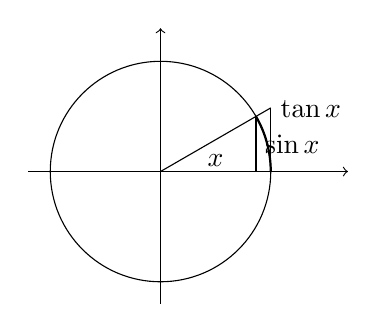
\begin{tikzpicture}[scale=1.4]
\draw[->] (-1.2,0)--(1.7,0);\draw[->](0,-1.2)--(0,1.3);\draw(0,0)circle(1);\draw(0,0)--(1,{tan(30)});\draw(1,0)--(1,{tan(30)});\draw({cos(30)},0)--({cos(30)},{sin(30)});\draw[thick](1,0) arc(0:30:1);\node[right] at (1,.57){$\tan x$};\node[right]at(.86,.25){$\sin x$};\node at(.5,.1){$x$};
\end{tikzpicture}\end{center}
Per $x>0$, $\sin x<x<\tan x$, dunque $\sin x/x<1$ e $x<\sin x/\cos x$ implica $\cos x<\sin x/x$.
Quindi
\[\cos x<\frac{\sin x}x<1.\]
Per il teorema del doppio confronto, dato che $\lim_{x\to0}\cos x=1$ e $\lim_{x\to0}1=1$, segue il limite.
% Pagina originale 54
\pagina{54}
\[\lim_{x\to0}\frac{1-\cos x}{x^2}=\frac12.\]
\begin{align*}
\lim_{x\to0}\frac{1-\cos x}{x^2}
&=\lim_{x\to0}\frac{(1-\cos x)(1+\cos x)}{x^2(1+\cos x)}\\
&=\lim_{x\to0}\frac{1-\cos^2x}{x^2(1+\cos x)}
=\lim_{x\to0}\frac{\sin^2x}{x^2}\frac1{1+\cos x}=\frac12.
\end{align*}
\[\lim_{x\to0}\frac{1-\cos x}x=\lim_{x\to0}\frac{1-\cos x}{x^2}x=\lim_{x\to0}\frac x2=0.\]
\[\lim_{x\to0}\frac{\tan x}x=\lim_{x\to0}\frac{\sin x}x\frac1{\cos x}=1.\]
\[\lim_{x\to0}\frac{\arcsin x}x=1,\qquad\lim_{x\to0}\frac{\arctan x}x=1.\]
Con $y=\arcsin x$, $x=\sin y$, si ha $\lim_{y\to0}y/\sin y=1^{-1}=1$.
Con $y=\arctan x$, $x=\tan y$, si ha $\lim_{y\to0}y/\tan y=1^{-1}=1$.
% Pagina originale 55
\pagina{55}\tit{4. Derivata}
$f:I\to\R$, $I$ intervallo, $x_0\in\mathring I$, $h\in\R$, $h\ne0$, $x_0+h\in I$.
Il rapporto incrementale è
\[\frac{f(x_0+h)-f(x_0)}{x_0+h-x_0}=\frac{f(x_0+h)-f(x_0)}h.\]
\[\lim_{h\to0}\frac{f(x_0+h)-f(x_0)}h=\lim_{x\to x_0}\frac{f(x)-f(x_0)}{x-x_0}.\]
$f$ è derivabile in $x_0\in\mathring I$ se esiste questo limite e appartiene a $\R$; si indica con
\[f'(x_0)=\lim_{h\to0}\frac{f(x_0+h)-f(x_0)}h=Df(x_0)=\frac{df}{dx}(x_0)=\dot f(x_0).\]
\tit{Funzione dotata di derivata in $x_0$}
$f$ si dice dotata di derivata in $x_0\in\mathring I$ se
\[\exists\lim_{x\to x_0}\frac{f(x)-f(x_0)}{x-x_0}=\pm\infty.\]
Una funzione dotata di derivata infinita non è derivabile.
Se $f'_+(x_0)\ne f'_-(x_0)$, non esiste $f'(x_0)$.
Infatti, se
\[\lim_{h\to0^+}\frac{f(x_0+h)-f(x_0)}h=f'_+(x_0)\in\R,\quad
\lim_{h\to0^-}\frac{f(x_0+h)-f(x_0)}h=f'_-(x_0)\in\R\]
e i due valori sono diversi, $f'(x_0)$ non esiste.
% Pagina originale 56
\pagina{56}
Se $f'_+(x_0)=f'_-(x_0)$, esiste $f'(x_0)$.
In maniera analoga, se esistono i due limiti laterali del rapporto incrementale in $\R$ e sono uguali,
\[f'(x_0)=f'_+(x_0)=f'_-(x_0).\]
\tit{Miglior approssimazione lineare in un punto}
$f:I\to\R$, $I$ intervallo, $x_0\in\mathring I$. Esiste $a_{x_0}\in\R$ tale che
\[f(x_0+h)=f(x_0)+a_{x_0}h+o(h),\]
ossia
\[f(x_0+h)-f(x_0)-a_{x_0}h=o(h),\qquad
\lim_{h\to0}\frac{f(x_0+h)-f(x_0)-a_{x_0}h}h=0.\]
\tit{Teorema: derivabilità e approssimazione lineare}
$f$ derivabile in $x_0$ se e solo se $f$ ha miglior approssimazione lineare in $x_0$; inoltre $a_{x_0}=f'(x_0)$.
\textit{Dimostrazione $\Leftarrow$.}
\[
0=\lim_{h\to0}\frac{f(x_0+h)-f(x_0)-a_{x_0}h}h
=\lim_{h\to0}\frac{f(x_0+h)-f(x_0)}h-a_{x_0}=f'(x_0)-a_{x_0},
\]
quindi $f'(x_0)=a_{x_0}$.
% Pagina originale 57
\pagina{57}
\textit{Dimostrazione $\Rightarrow$.}
\[\lim_{h\to0}\frac{f(x_0+h)-f(x_0)}h=f'(x_0)=a\]
implica
\[\lim_{h\to0}\left(\frac{f(x_0+h)-f(x_0)}h-a\right)=0,
\quad\lim_{h\to0}\frac{f(x_0+h)-f(x_0)-ah}h=0.\]
Quindi $a=a_{x_0}$, cioè $a_{x_0}=f'(x_0)$.
\tit{Osservazioni sulla miglior approssimazione lineare}
$f$ ha miglior approssimazione lineare in $x_0$ se esiste $f'(x_0)\in\R$ tale che
\[f(x_0+h)=f(x_0)+f'(x_0)h+o(h).\]
Cioè
\[\lim_{h\to0}\frac{f(x_0+h)-f(x_0)-f'(x_0)h}h=0
\iff\lim_{x\to x_0}\frac{f(x)-f(x_0)-f'(x_0)(x-x_0)}{x-x_0}=0.\]
Pertanto
\[f(x)-f(x_0)-f'(x_0)(x-x_0)=o(x-x_0),\]
e $f(x)-[f(x_0)+f'(x_0)(x-x_0)]\approx0$.
La retta $y=f(x_0)+f'(x_0)(x-x_0)$ è la miglior approssimazione lineare della funzione $f$ in $x_0$.
\nota{Nelle ultime due righe dell'originale compare un segno meno davanti al termine con $f'(x_0)$, in contrasto con i passaggi precedenti.}
% Pagina originale 58
\pagina{58}\tit{Derivabile implica continua}
$f:I\to\R$, $x_0\in\mathring I$: se $f$ è derivabile in $x_0$, è continua in $x_0$.
\textit{Dimostrazione.} Dalla miglior approssimazione lineare,
\[f(x)-f(x_0)-f'(x_0)(x-x_0)=o(x-x_0),\]
quindi $f(x)-f(x_0)=o(x-x_0)+f'(x_0)(x-x_0)$.
Poiché $o(x-x_0)/(x-x_0)\to0$ e $x-x_0\to0$, si ha $o(x-x_0)\to0$; inoltre $f'(x_0)(x-x_0)\to0$.
Dunque $\lim_{x\to x_0}f(x)=f(x_0)$.
\tit{Derivabile a destra e a sinistra implica continua}
$f:I\to\R$, $x_0\in I$: se $f$ è derivabile a destra e a sinistra in $x_0$, è continua in $x_0$.
\textit{Dimostrazione.}
\[f(x)-f(x_0)-f'_+(x_0)(x-x_0)=o(x-x_0)\quad(x\to x_0^+).\]
Allora $\lim_{x\to x_0^+}(f(x)-f(x_0))=0$, perché entrambi i termini $o(x-x_0)$ e $f'_+(x_0)(x-x_0)$ tendono a zero. Analogamente $\lim_{x\to x_0^-}f(x)=f(x_0)$, e quindi $\lim_{x\to x_0}f(x)=f(x_0)$.
% Pagina originale 59
\pagina{59}\tit{Punti non derivabili}
\begin{enumerate}
\item Punto angoloso: $f'_+(x_0)\ne f'_-(x_0)$; oppure esiste una derivata laterale finita e il limite del rapporto incrementale dall'altro lato è $\pm\infty$.
\item Punto cuspidale o cuspide:
\[\lim_{x\to x_0^+}\frac{f(x)-f(x_0)}{x-x_0}=\pm\infty=-\lim_{x\to x_0^-}\frac{f(x)-f(x_0)}{x-x_0}.\]
\item Punto di flesso verticale:
\[\lim_{x\to x_0}\frac{f(x)-f(x_0)}{x-x_0}=\pm\infty.\]
La funzione è dotata di derivata in $x_0$.
\end{enumerate}
\begin{center}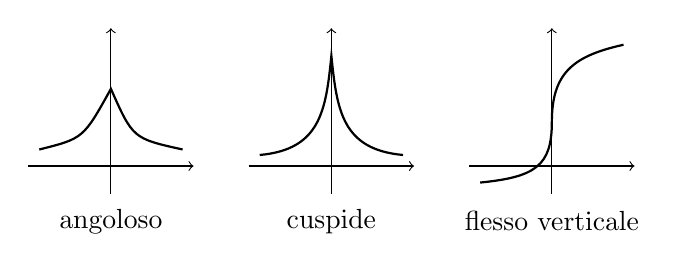
\begin{tikzpicture}[scale=.7]
\foreach \s in {0,4,8}{\draw[->](\s-1.5,0)--(\s+1.5,0);\draw[->](\s,-.5)--(\s,2.5);}
\draw[thick](-1.3,.3)..controls(-.5,.5)..(0,1.4)..controls(.4,.5)..(1.3,.3);
\draw[thick](2.7,.2)..controls(3.8,.3)and(3.9,1)..(4,2)..controls(4.1,1)and(4.2,.3)..(5.3,.2);
\draw[thick](6.7,-.3)..controls(7.7,-.2)and(8,0)..(8,.8)..controls(8,1.7)and(8.4,2)..(9.3,2.2);
\node at(0,-1){angoloso};\node at(4,-1){cuspide};\node at(8,-1){flesso verticale};
\end{tikzpicture}\end{center}
\tit{Regole di derivazione}
Additività: $D(f+g)=D(f)+D(g)$.
Linearità: $D(kf)=kD(f)$.
\textit{Somma.}
\begin{align*}
D(f+g)(x_0)&=\lim_{h\to0}\left[\frac{f(x_0+h)-f(x_0)}h+\frac{g(x_0+h)-g(x_0)}h\right]\\
&=f'(x_0)+g'(x_0).
\end{align*}
% Pagina originale 60
\pagina{60}\tit{Prodotto: regola di Leibniz}
\[(fg)'(x_0)=f'(x_0)g(x_0)+f(x_0)g'(x_0).\]
\textit{Dimostrazione.}
\begin{align*}
\lim_{x\to x_0}\frac{f(x)g(x)-f(x_0)g(x_0)}{x-x_0}
&=\lim_{x\to x_0}\frac{f(x)g(x)-f(x)g(x_0)+f(x)g(x_0)-f(x_0)g(x_0)}{x-x_0}\\
&=\lim_{x\to x_0}\left[f(x)\frac{g(x)-g(x_0)}{x-x_0}+g(x_0)\frac{f(x)-f(x_0)}{x-x_0}\right]\\
&=f(x_0)g'(x_0)+g(x_0)f'(x_0).
\end{align*}
\tit{Quoziente}
\[\left(\frac fg\right)'(x_0)=\frac{f'(x_0)g(x_0)-f(x_0)g'(x_0)}{[g(x_0)]^2}.\]
L'esistenza di $f'$ e $g'$ implica quella di $(fg)'$. Non è vero il contrario.
Esempio: non esistono $(\sqrt{x})'(0)$ e $(\sqrt{x})'(0)$ come derivate finite, ma esiste $(\sqrt{x}\sqrt{x})'(0)$.
% Pagina originale 61
\pagina{61}\tit{Derivata di funzione composta}
$f:I\to\R$, $g:J\to\R$, $f(I)\subset J$, $x_0\in I$, esistono $f'(x_0)$ e $g'(f(x_0))$. Allora $g\circ f$ è derivabile in $x_0$ e
\[D(g\circ f)(x_0)=Dg(f(x_0))\,Df(x_0).\]
\textit{Dimostrazione} (ipotesi aggiuntiva: esiste un intorno $U$ di $x_0$ tale che per ogni $x\in U\setminus\{x_0\}$, $f(x)\ne f(x_0)$).
\begin{align*}
\frac{(g\circ f)(x)-(g\circ f)(x_0)}{x-x_0}&=\frac{g(f(x))-g(f(x_0))}{x-x_0},\\
\lim_{x\to x_0}\frac{g(f(x))-g(f(x_0))}{x-x_0}
&=\lim_{x\to x_0}\frac{g(f(x))-g(f(x_0))}{f(x)-f(x_0)}\frac{f(x)-f(x_0)}{x-x_0}\\
&=g'(f(x_0))f'(x_0).
\end{align*}
\tit{Derivata della funzione inversa}
$f:I\to\R$ invertibile: esiste $f^{-1}$ con $f^{-1}(f(x))=x$ e $f(f^{-1}(y))=y$.
Siano $x_0\in I$, $f\in C^0(I)$, $f'(x_0)\ne0$, $f^{-1}:f(I)\to I$, $f^{-1}\in C^0(f(I))$.
Allora $f^{-1}$ è derivabile in $f(x_0)$ e
\[(f^{-1})'(f(x_0))=\frac1{f'(x_0)}.\]
\textit{Dimostrazione.} Con $y_0=f(x_0)$,
\begin{align*}
\lim_{y\to y_0}\frac{f^{-1}(y)-f^{-1}(y_0)}{y-y_0}
&=\lim_{x\to x_0}\frac{f^{-1}(f(x))-f^{-1}(f(x_0))}{f(x)-f(x_0)}\\
&=\lim_{x\to x_0}\frac{x-x_0}{f(x)-f(x_0)}=\frac1{f'(x_0)}.
\end{align*}
% Pagina originale 62
\pagina{62}\tit{Punto stazionario}
$f:I\to\R$, $x_0\in I$, esiste $f'(x_0)$. Se $f'(x_0)=0$, $x_0$ è punto stazionario.
\tit{Punto critico}
$x_0\in I$ è punto critico se $f'(x_0)=0$ (punto stazionario), oppure $f'(x_0)$ non esiste.
\tit{Teorema di Fermat}
$f:A\to\R$, $I\subset A$ intervallo, $x_0\in\mathring I$, esiste $f'(x_0)$. Se $x_0$ è estremale, allora è stazionario (critico).
\textit{Dimostrazione per assurdo.} Supponiamo $f'(x_0)\ne0$.
\begin{enumerate}
\item Se $f'(x_0)>0$, allora $\lim_{x\to x_0}(f(x)-f(x_0))/(x-x_0)>0$. Pertanto, vicino a $x_0$, $f(x)>f(x_0)$ per $x>x_0$ e $f(x)<f(x_0)$ per $x<x_0$: $x_0$ non è punto di massimo o minimo.
\item Se $f'(x_0)<0$, analogamente $f(x)>f(x_0)$ per $x<x_0$ e $f(x)<f(x_0)$ per $x>x_0$: $x_0$ non è punto di massimo o minimo.
\end{enumerate}
% Pagina originale 63
\pagina{63}\tit{Teorema di Rolle}
$f:A\to\R$, $[a,b]\subset A$, $f\in C^0([a,b])$, $f$ derivabile in $(a,b)$, $f(a)=f(b)$.
Allora esiste $x_0\in(a,b)$ tale che $f'(x_0)=0$.
\begin{center}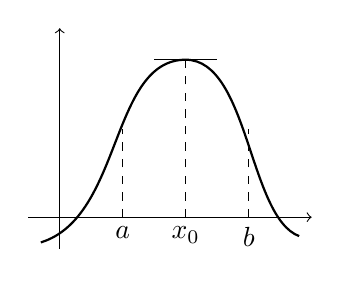
\begin{tikzpicture}[scale=.8]\draw[->](-.5,0)--(4,0);\draw[->](0,-.5)--(0,3);\draw[thick](-.3,-.4)..controls(1,0)and(.8,2.5)..(2,2.5)..controls(3,2.5)and(3,0)..(3.8,-.3);\draw[dashed](1,0)--(1,1.4)(2,0)--(2,2.5)(3,0)--(3,1.4);\draw(1.5,2.5)--(2.5,2.5);\node[below]at(1,0){$a$};\node[below]at(2,0){$x_0$};\node[below]at(3,0){$b$};\end{tikzpicture}\end{center}
\textit{Dimostrazione.} La funzione è limitata e continua; usando Weierstrass e il teorema dei valori intermedi, $f([a,b])=[m,M]$.
\begin{enumerate}
\item Se $f(a)=m$ e $f(b)=M$ (o viceversa), essendo $f(a)=f(b)$, si ha $m=M$. Quindi $f$ è costante e $f'(x)=0$ per ogni $x\in(a,b)$.
\item In caso contrario si ha un punto estremale $x_0\in(a,b)$, e per Fermat $f'(x_0)=0$.
\end{enumerate}
% Pagina originale 64
\pagina{64}\tit{Teorema di Cauchy}
$f,g:A\to\R$, $[a,b]\subset A$, $f,g\in C^0([a,b])$, entrambe derivabili in $(a,b)$ e $g'(x)\ne0$ per ogni $x\in(a,b)$.
Allora esiste $c\in(a,b)$ tale che
\[\frac{f(b)-f(a)}{g(b)-g(a)}=\frac{f'(c)}{g'(c)}.\]
\textit{Dimostrazione.} Definiamo
\[h(x)=[g(b)-g(a)]f(x)-[f(b)-f(a)]g(x).\]
$h\in C^0([a,b])$ ed è derivabile in $(a,b)$.
\begin{align*}
h(a)&=g(b)f(a)-g(a)f(a)-f(b)g(a)+f(a)g(a)\\&=f(a)g(b)-f(b)g(a),\\
h(b)&=g(b)f(b)-g(a)f(b)-f(b)g(b)+f(a)g(b)\\&=f(a)g(b)-g(a)f(b).
\end{align*}
Poiché $h(a)=h(b)$ possiamo applicare Rolle: esiste $c\in(a,b)$ con $h'(c)=0$.
Dunque
\[f'(c)[g(b)-g(a)]=g'(c)[f(b)-f(a)],\quad\frac{f'(c)}{g'(c)}=\frac{f(b)-f(a)}{g(b)-g(a)}.\]
% Pagina originale 65
\pagina{65}\tit{Teorema di Lagrange}
$f:A\to\R$, $[a,b]\subset A$, $f\in C^0([a,b])$, $f$ derivabile in $(a,b)$.
Allora esiste $c\in(a,b)$ tale che
\[\frac{f(b)-f(a)}{b-a}=f'(c).\]
\textit{Dimostrazione.} Applichiamo Cauchy con $g(x)=x$:
\[\frac{f(b)-f(a)}{g(b)-g(a)}=\frac{f'(c)}{g'(c)}\implies\frac{f(b)-f(a)}{b-a}=f'(c).\]
\textit{Osservazione.} $(f(b)-f(a))/(b-a)=(y_b-y_a)/(x_b-x_a)$ è il coefficiente angolare della retta secante.
\begin{center}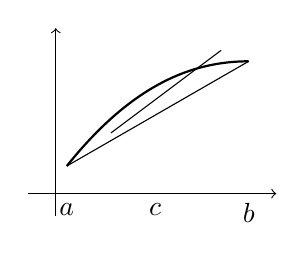
\begin{tikzpicture}[scale=.7]\draw[->](-.5,0)--(4,0);\draw[->](0,-.4)--(0,3);\draw[thick](.2,.5)..controls(1.4,2)and(2.5,2.4)..(3.5,2.4);\draw(.2,.5)--(3.5,2.4);\draw(1,1.1)--(3,2.6);\node[below]at(.2,0){$a$};\node[below]at(1.8,0){$c$};\node[below]at(3.5,0){$b$};\end{tikzpicture}\end{center}
\tit{Corollario: derivata nulla implica funzione costante}
Se $f'(x)=0$ per ogni $x\in(a,b)$, allora $f(x)=k$.
\textit{Dimostrazione.} Fissati $x_1,x\in[a,b]$, $x_1\ne x$, se $x<x_1$, $[x,x_1]\subset[a,b]$ e per Lagrange esiste $c\in(x,x_1)$ con
\[0=f'(c)=\frac{f(x_1)-f(x)}{x_1-x},\]
quindi $f(x_1)=f(x)$.
% Pagina originale 66
\pagina{66}
Se invece $x>x_1$, $[x_1,x]\subset[a,b]$ e per Lagrange esiste $c\in(x_1,x)$ con
\[0=f'(c)=\frac{f(x)-f(x_1)}{x-x_1},\]
quindi $f(x)=f(x_1)$. In conclusione $f$ è costante su $[a,b]$.
\tit{Caratterizzazione della monotonia mediante il segno della derivata}
$f:A\to\R$, $[a,b]\subset A$, $f\in C^0([a,b])$, $f$ derivabile in $(a,b)$.
\[f\text{ monotona crescente su }[a,b]\iff f'(x)\ge0\quad\forall x\in(a,b).\]
\textit{Dimostrazione $\Rightarrow$, per assurdo.} Supponiamo che esista $x_0\in(a,b)$ con $f'(x_0)<0$.
Esiste allora un intorno $U$ di $x_0$ contenuto in $(a,b)$ tale che per ogni $x\in U\setminus\{x_0\}$,
\[\frac{f(x)-f(x_0)}{x-x_0}<0.\]
Quindi $f(x)>f(x_0)$ se $x<x_0$ e $f(x)<f(x_0)$ se $x>x_0$. Ciò contraddice la proprietà $x_1\le x_2\implies f(x_1)\le f(x_2)$.
% Pagina originale 67
\pagina{67}
\textit{Dimostrazione $\Leftarrow$.} Prendiamo $x_1,x_2\in[a,b]$ con $x_1<x_2$. Allora $[x_1,x_2]\subset[a,b]$ e per Lagrange esiste $c\in(x_1,x_2)$ tale che
\[f'(c)(x_2-x_1)=f(x_2)-f(x_1).\]
$f'(c)\ge0$ e $x_2-x_1>0$ implicano $f(x_2)-f(x_1)\ge0$, cioè $f(x_1)\le f(x_2)$.
\tit{Derivata positiva implica stretta crescita}
Se $f'(x)>0$ per ogni $x\in(a,b)$, $f$ è strettamente crescente.
\textit{Dimostrazione.} Per $x_1<x_2$, Lagrange dà $f'(c)(x_2-x_1)=f(x_2)-f(x_1)$. Essendo entrambi i fattori positivi, $f(x_1)<f(x_2)$.
\textit{Osservazione.} La stretta crescita non implica $f'(x)>0$ ovunque.
Esempio: $x^3$ è strettamente crescente in $\R$, ma $D(x^3)=3x^2>0$ soltanto per $x\ne0$ e $f'(0)=0$.
\begin{center}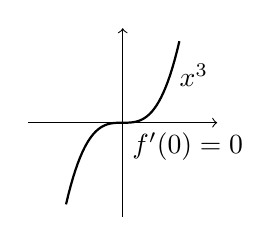
\begin{tikzpicture}[scale=.6]\draw[->](-2,0)--(2,0);\draw[->](0,-2)--(0,2);\draw[thick,domain=-1.2:1.2,samples=50]plot(\x,{\x^3});\node[right]at(1,1){$x^3$};\node[below right]at(0,0){$f'(0)=0$};\end{tikzpicture}\end{center}
% Pagina originale 68
\pagina{68}\tit{5. Primitiva di una funzione}
$f:I\to\R$. Una funzione $F:I\to\R$ è una primitiva di $f$ se $F'(x)=f(x)$ per ogni $x\in I$.
\[\int f(x)\,dx:=\{F:I\to\R\mid F'(x)=f(x)\ \forall x\in I\}.\]
$f$ è la funzione integranda.
\tit{Le primitive distano di una costante}
Se $F_1,F_2:I\to\R$ sono primitive di $f$, esiste $c\in\R$ tale che $F_1-F_2=c$.
\textit{Dimostrazione.} $H(x):=F_1(x)-F_2(x)$ è derivabile in $I$ e $H'(x)=f(x)-f(x)=0$. Dunque $H$ è costante.
\tit{Linearità dell'integrale indefinito}
$f,g:I\to\R$ ammettono primitive. Per ogni $\alpha,\beta\in\R$,
\[\int(\alpha f+\beta g)(x)\,dx=\alpha\int f(x)\,dx+\beta\int g(x)\,dx.\]
\textit{Dimostrazione.} Se $F'=f$ e $G'=g$, allora $(\alpha F+\beta G)'=\alpha F'+\beta G'=\alpha f+\beta g$.
% Pagina originale 69
\pagina{69}\tit{Regole di integrazione}
\textbf{1. Integrazione per parti}
\[\int f(x)g'(x)\,dx=f(x)g(x)-\int f'(x)g(x)\,dx.\]
Deriva da $[f(x)g(x)]'=f'(x)g(x)+f(x)g'(x)$:
\begin{align*}
\int[f(x)g(x)]'\,dx&=\int\bigl(f'(x)g(x)+f(x)g'(x)\bigr)\,dx,\\
f(x)g(x)&=\int f'(x)g(x)\,dx+\int f(x)g'(x)\,dx,
\end{align*}
da cui la formula.
\textbf{2. Integrazione per sostituzione}
\[\int f(g(x))g'(x)\,dx=F(g(x))+c,\qquad F'=f.\]
Deriva da $[F(g(x))]'=F'(g(x))g'(x)=f(g(x))g'(x)$.
Ponendo $y=g(x)$ e $dy=g'(x)dx$,
\[\int f(g(x))g'(x)\,dx=\int f(y)\,dy=F(y)+c=F(g(x))+c.\]
% Pagina originale 70
\pagina{70}\tit{Teorema di de l'Hôpital}
$f,g:(a,b)\to\R$, $-\infty\le a<b\le+\infty$, derivabili in $(a,b)$, con $\lim_{x\to a^+}f(x),\lim_{x\to a^+}g(x)$ entrambi zero oppure infiniti.
Esiste un intorno destro $U$ di $a$ tale che $g'(x)\ne0$ per ogni $x\in U\cap(a,b)$.
Se $\lim_{x\to a^+}f'(x)/g'(x)=\ell$, allora $g(x)\ne0$ vicino ad $a$ e
\[\lim_{x\to a^+}\frac{f(x)}{g(x)}=\ell.\]
\textit{Dimostrazione.} Supponiamo $f,g$ infinitesime per $x\to a^+$. Estendiamole su $[a,b)$:
\[\widetilde f(x)=\begin{cases}f(x)&x\in(a,b),\\0&x=a,\end{cases}\qquad
\widetilde g(x)=\begin{cases}g(x)&x\in(a,b),\\0&x=a.\end{cases}\]
Sono derivabili in $(a,b)$ e continue su $[a,c]$, $a<c<b$.
Scegliamo $c>a$ tale che $g'(x)\ne0$ per ogni $x\in(a,c)$. Applichiamo Cauchy su $[a,x]$:
\[\exists\xi(x)\in(a,x):\quad\frac{\widetilde f'(\xi(x))}{\widetilde g'(\xi(x))}
=\frac{\widetilde f(x)-\widetilde f(a)}{\widetilde g(x)-\widetilde g(a)}=\frac{\widetilde f(x)}{\widetilde g(x)}.\]
% Pagina originale 71
\pagina{71}
Essendo continue,
\[\lim_{x\to a^+}\frac{\widetilde f(x)}{\widetilde g(x)}=\lim_{x\to a^+}\frac{f(x)}{g(x)}.\]
Quindi, ponendo $y=\xi(x)$,
\[\lim_{x\to a^+}\frac{f(x)}{g(x)}=\lim_{x\to a^+}\frac{f'(\xi(x))}{g'(\xi(x))}=\lim_{y\to a^+}\frac{f'(y)}{g'(y)}=\ell.\]
\tit{Applicazioni del teorema di de l'Hôpital}
\[\exists\lim_{x\to x_0}f'(x)=\ell\Longrightarrow\exists f'(x_0)=\ell.\]
\textit{Dimostrazione.}
\[\lim_{x\to x_0}\frac{f(x)-f(x_0)}{x-x_0}\quad[0/0]\overset H=\lim_{x\to x_0}\frac{f'(x)}1=\ell=f'(x_0).\]
\nota{Pagina 71: dopo Hôpital il manoscritto reca $f'(x)-f'(x_0)$ al numeratore, ma la derivata della costante $f(x_0)$ è zero. La continuità in $x_0$ è utilizzata nella forma $0/0$.}
\tit{Convessità}
\[\alpha:[0,1]\to[x_1,x_2],\quad\lambda\mapsto x_1+\lambda(x_2-x_1),\quad x_1<x_2;\qquad\alpha([0,1])=[x_1,x_2].\]
\[\alpha(\lambda)=x_1+\lambda(x_2-x_1)=x_1+\lambda x_2-\lambda x_1=(1-\lambda)x_1+\lambda x_2.\]
La secante $s$ per $(x_1,f(x_1))$ e $(x_2,f(x_2))$ ha equazioni
\[\frac{y-f(x_2)}{f(x_1)-f(x_2)}=\frac{x-x_2}{x_1-x_2},\quad
s(x)=f(x_1)+(x-x_1)\frac{f(x_2)-f(x_1)}{x_2-x_1}.\]
\begin{center}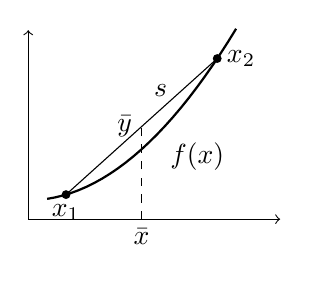
\begin{tikzpicture}[scale=.8]\draw[->](0,0)--(4,0);\draw[->](0,0)--(0,3);\draw[thick,domain=.3:3.3]plot(\x,{.25*\x*\x+.3});\draw(.6,.39)--(3,2.55);\fill(.6,.39)circle(2pt)node[below]{$x_1$};\fill(3,2.55)circle(2pt)node[right]{$x_2$};\draw[dashed](1.8,0)--(1.8,1.47);\node[below]at(1.8,0){$\bar x$};\node[left]at(1.8,1.47){$\bar y$};\node[right]at(2.1,1){$f(x)$};\node[above]at(2.1,1.8){$s$};\end{tikzpicture}\end{center}
% Pagina originale 72
\pagina{72}
Nelle funzioni convesse $f(\bar x)\le\bar y=s(\bar x)$, con
\[s:x\mapsto f(x_1)+(x-x_1)\frac{f(x_2)-f(x_1)}{x_2-x_1}.\]
Per $\bar x\in[x_1,x_2]$ esiste $\bar\lambda=\alpha^{-1}(\bar x)$:
\[\bar x=(1-\bar\lambda)x_1+\bar\lambda x_2,\quad\bar x-x_1=\bar\lambda(x_2-x_1).\]
\begin{align*}s(\bar x)&=f(x_1)+\bar\lambda(x_2-x_1)\frac{f(x_2)-f(x_1)}{x_2-x_1}\\&=f(x_1)+\bar\lambda(f(x_2)-f(x_1))=(1-\bar\lambda)f(x_1)+\bar\lambda f(x_2).\end{align*}
Quindi $f((1-\lambda)x_1+\lambda x_2)\le(1-\lambda)f(x_1)+\lambda f(x_2)$.
Nelle funzioni concave $f(\bar x)\ge s(\bar x)$, quindi
\[f((1-\lambda)x_1+\lambda x_2)\ge(1-\lambda)f(x_1)+\lambda f(x_2).\]
\tit{Conseguenze della convessità}
Se $f:I\to\R$ è convessa:
\begin{enumerate}\item Per ogni $x\in\mathring I$ esistono $f'_+(x),f'_-(x)\in\R$.
\item Per ogni $x\in\mathring I$, $f'_+(x)\ge f'_-(x)$.
\item $f'_+$ e $f'_-$ sono crescenti.\end{enumerate}
% Pagina originale 73
\pagina{73}\tit{Derivata seconda}
Se esiste $(f')'(x_0)$, esiste $f''(x_0)\in\R$.
$f:I\to\R$ derivabile in un intervallo $J\subset I$; $f':J\to\R$, $x_0\in J$.
Se $f'$ è derivabile,
\[\exists\lim_{x\to x_0}\frac{f'(x)-f'(x_0)}{x-x_0}=\ell\in\R,\quad
\ell=(f')'(x_0)=f''(x_0)=D^2f(x_0)=\ddot f(x_0)=\frac{d^2f}{dx^2}(x_0).\]
\tit{Classi $C^0,C^1,C^n,C^\infty$}
\begin{align*}
C^0(J)&:=\{f:J\to\R\mid f\text{ continua}\},\\
C^1(J)&:=\{f:J\to\R\mid f\text{ derivabile in }J,\ f'\in C^0(J)\},\\
C^2(J)&:=\{f:J\to\R\mid f\text{ derivabile due volte in }J,\ f''\in C^0(J),\ f'\in C^1(J)\},\\
C^n(J)&:=\{f:J\to\R\mid f\text{ derivabile }n\text{ volte in }J,\ f^{(n)}\in C^0(J),\\&\hspace{25mm}f^{(n-1)}\in C^1(J),\ldots,f'\in C^{n-1}(J)\},\\
C^\infty(J)&:=\{f:J\to\R\mid f\text{ derivabile infinite volte in }J,\ \forall n\in\N:\ f^{(n)}\in C^0(J)\}.
\end{align*}
\textit{Osservazione.} $f\in C^n(J)$ implica $f\in C^{n-1}(J),C^{n-2}(J),\ldots,C^0(J)$.
\[C^\infty\subsetneq C^n\subsetneq C^{n-1}\subsetneq\cdots\subsetneq C^1\subsetneq C^0.\]
% Pagina originale 74
\pagina{74}\tit{Convessità e derivata seconda}
\[f\text{ convessa}\iff f''>0.\]
\textit{Dimostrazione (come negli appunti).} $f$ convessa se e solo se $f'$ crescente; $f'$ crescente implica $(f')'>0$, quindi $f''>0$.
\nota{Pagina 74: il manoscritto riporta disuguaglianze strette; per la convessità non stretta il criterio corretto, per funzioni due volte derivabili, è $f''\ge0$.}
\tit{Punto di flesso}
$f:(a,b)\to\R$. $x_0\in(a,b)$ è punto di flesso se $f$ è strettamente convessa/concava in un intorno sinistro $I^-(x_0)\cap(a,b)$ ed è strettamente concava/convessa in un intorno destro $I^+(x_0)\cap(a,b)$.
\[x_0\text{ punto di flesso}\Longrightarrow f''(x_0)=0.\]
\textit{Dimostrazione.} $f'$ crescente a destra e decrescente a sinistra: $f'$ ha un massimo in $x_0$, quindi $x_0$ è punto estremale. Per il teorema di Fermat $f''(x_0)=0$.
\tit{Tipi di punto di flesso}
\begin{itemize}\item Tangente orizzontale se $f'(x_0)=0$.\item Tangente verticale se $f'(x_0)=\pm\infty$.\item Ascendente se $f'(x_0)>0$.\item Discendente se $f'(x_0)<0$.\end{itemize}
% Pagina originale 75
\pagina{75}\tit{Derivate elementari}
\textbf{1. Potenza:} $D x^\alpha=\alpha x^{\alpha-1}$.
\[\lim_{h\to0}\frac{(x+h)^\alpha-x^\alpha}{h}=\lim_{h\to0}\frac{x^\alpha[(1+h/x)^\alpha-1]}{(h/x)x}=\alpha x^{\alpha-1}.\]
\textbf{2. Esponenziale:} $D a^x=a^x\log a$.
\[\lim_{h\to0}\frac{a^{x+h}-a^x}{h}=\lim_{h\to0}a^x\frac{a^h-1}{h}=a^x\log a.\]
\textbf{3. Logaritmo:} $D\log_a x=1/(x\log a)$.
\begin{align*}\lim_{h\to0}\frac{\log_a(x+h)-\log_a x}{h}&=\lim_{h\to0}\frac{\log_a[x(1+h/x)]-\log_a x}{h}\\&=\lim_{h\to0}\frac{\log_a(1+h/x)}{(h/x)x}=\frac1x\log_a e=\frac1{x\log a}.\end{align*}
\textbf{4. Seno:} $D\sin x=\cos x$.
\[\frac{\sin(x+h)-\sin x}{h}=\frac{\sin x\cos h+\sin h\cos x-\sin x}{h}=\sin x\frac{\cos h-1}{h}+\frac{\sin h}{h}\cos x\longrightarrow\cos x.\]
\textbf{5.} $D\cos x=-\sin x$.\quad
\textbf{6.} $D\tan x=1/\cos^2x=1+\tan^2x$.
\textbf{7.} $D\arcsin x=1/\sqrt{1-x^2}$; $D\arccos x=-1/\sqrt{1-x^2}$.
\textbf{8.} $D\arctan x=1/(1+x^2)$; $D\operatorname{arccot}x=-1/(1+x^2)$.
% Pagina originale 76
\pagina{76}\tit{Formula di Taylor}
$f:I\to\R$, $x_0\in I$, esiste $f'(x_0)\in\R$ se e solo se
\[f(x)=f(x_0)+f'(x_0)(x-x_0)+o(x-x_0).\]
L'espressione lineare è $P_1(x)$. Analogamente, per $f$ derivabile $n$ volte,
\[P_n(x)=\sum_{k=0}^n\frac{f^{(k)}(x_0)}{k!}(x-x_0)^k
=f(x_0)+f'(x_0)(x-x_0)+\frac{f''(x_0)}2(x-x_0)^2+\cdots.\]
\textbf{1.} $P_n(x_0)=f(x_0)$, $P'_n(x_0)=f'(x_0)$, $\ldots$, $P_n^{(k)}(x_0)=f^{(k)}(x_0)$.
\textit{Dimostrazione.}
\[P_n(x_0)=f(x_0)+f'(x_0)(x_0-x_0)+\cdots=f(x_0),\]
\[P'_n(x_0)=f'(x_0)+f''(x_0)(x_0-x_0)+\cdots=f'(x_0).\]
\begin{align*}
P_n''(x_0)&=\left.\frac d{dx}\left(\sum_{k=1}^n\frac{f^{(k)}(x_0)}{k!}k(x-x_0)^{k-1}\right)\right|_{x=x_0}\\
&=\left.\frac d{dx}\left(\sum_{k=0}^{n-1}\frac{f^{(k+1)}(x_0)}{k!}(x-x_0)^k\right)\right|_{x=x_0}\\
&=\left.\sum_{k=1}^{n-1}\frac{f^{(k+1)}(x_0)}{(k-1)!}(x-x_0)^{k-1}\right|_{x=x_0}\\
&=\left.\sum_{k=0}^{n-2}\frac{f^{(k+2)}(x_0)}{k!}(x-x_0)^k\right|_{x=x_0}=f''(x_0)+0+\cdots=f''(x_0).
\end{align*}
Si procede analogamente per le successive derivate.
% Pagina originale 77
\pagina{77}
\textbf{2.} $f(x)-P_n(x)=o((x-x_0)^n)$.
\textit{Ipotesi.} $f:I\to\R$, $x_0\in I$, $f$ derivabile $n$ volte in $x_0$.
\[f(x)-P_n(x)=o((x-x_0)^n),\quad\text{cioè}\quad\lim_{x\to x_0}\frac{f(x)-P_n(x)}{(x-x_0)^n}=0.\]
\textit{Dimostrazione.} Esiste un intorno $U$ di $x_0$ in cui sono definite tutte le derivate di ordine $n-1,n-2,\ldots,2,1$: per ogni $x\in U$, $f^{(k)}(x)\in\R$ per $k\in\{1,\ldots,n-1\}$.
Poniamo $g(x)=(x-x_0)^n$; $g'(x)=n(x-x_0)^{n-1}\ne0$ per $x\ne x_0$, e $g^{(k)}(x)\ne0$ per $x\ne x_0$, $k=1,\ldots,n$.
Possiamo quindi applicare de l'Hôpital:
\begin{align*}
\lim_{x\to x_0}\frac{f(x)-P_n(x)}{(x-x_0)^n}
&\overset H=\lim_{x\to x_0}\frac{f'(x)-P'_n(x)}{n(x-x_0)^{n-1}}\\
&\overset H=\cdots=\lim_{x\to x_0}\frac{f^{(n-1)}(x)-P_n^{(n-1)}(x)}{n(n-1)\cdots2(x-x_0)}.
\end{align*}
\[P_n^{(n-1)}(x)=f^{(n-1)}(x_0)+\frac{f^{(n)}(x_0)}{1!}(x-x_0).\]
Il limite diventa
\[\lim_{x\to x_0}\frac{f^{(n-1)}(x)-f^{(n-1)}(x_0)-f^{(n)}(x_0)(x-x_0)}{n(n-1)\cdots2(x-x_0)}.\]
% Pagina originale 78
\pagina{78}
\begin{align*}
&\lim_{x\to x_0}\frac1{n!}\left(\frac{f^{(n-1)}(x)-f^{(n-1)}(x_0)}{x-x_0}-f^{(n)}(x_0)\right)\\
&=\frac1{n!}\left(\lim_{x\to x_0}\frac{f^{(n-1)}(x)-f^{(n-1)}(x_0)}{x-x_0}-f^{(n)}(x_0)\right)=\frac1{n!}\cdot0=0.
\end{align*}
\tit{Caratterizzazione dei punti estremali tramite $f^{(n)}$}
$f:I\to\R$, $x_0\in I$, $f$ derivabile $n$ volte in $x_0$.
Se $f^{(n)}(x_0)\ne0$ e $f^{(i)}(x_0)=0$ per $i=1,\ldots,n-1$:
\begin{itemize}\item $n$ dispari: $x_0$ non è estremale.
\item $n$ pari e $f^{(n)}(x_0)>0$: $x_0$ minimo locale forte.
\item $n$ pari e $f^{(n)}(x_0)<0$: $x_0$ massimo locale forte.\end{itemize}
\textit{Dimostrazione.}
\begin{align*}
f(x)&=\sum_{k=0}^n\frac{f^{(k)}(x_0)}{k!}(x-x_0)^k+o((x-x_0)^n)\\
&=f(x_0)+f'(x_0)(x-x_0)+\cdots+\frac{f^{(n)}(x_0)}{n!}(x-x_0)^n+o((x-x_0)^n)\\
&=f(x_0)+\frac{f^{(n)}(x_0)}{n!}(x-x_0)^n+o((x-x_0)^n).
\end{align*}
Supponiamo $f(x)>f(x_0)$ per ogni $x\in I(x_0)\setminus\{x_0\}$:
\[f(x)-f(x_0)>0,\quad
f(x)-f(x_0)=(x-x_0)^n\left[\frac{f^{(n)}(x_0)}{n!}+\frac{o((x-x_0)^n)}{(x-x_0)^n}\right].\]
Se $n$ pari, $(x-x_0)^n>0$ per $x\ne x_0$ e
\[\frac{f^{(n)}(x_0)}{n!}+\frac{o((x-x_0)^n)}{(x-x_0)^n}\longrightarrow\frac{f^{(n)}(x_0)}{n!}>0.\]
\nota{Pagina 78: nella catena della dimostrazione il manoscritto usa $>$ al posto dell'uguaglianza dello sviluppo; sopra è resa esplicita l'identità di Taylor.}
% Pagina originale 79
\pagina{79}\tit{Polinomio di Maclaurin}
\[P_{n,0}(x)=\sum_{k=0}^n\frac{f^{(k)}(0)}{k!}x^k,\qquad f(x)=P_{n,0}(x)+o(x^n).\]
\tit{Integrale di Riemann}
\[R:=\{(x,y):x\in[a,b],\ 0\le y\le f(x)\}.\]
$R$ rettangolabile.
\[D([a,b]):=\{(t_i)_{i=0}^n:\ \forall i,\ t_i\in[a,b],\ a=t_0<t_1<\cdots<t_n=b\}.\]
$D$ è una suddivisione di $[a,b]$.
\[\mathcal D([a,b]):=\{D\in\mathcal P([a,b]):D\text{ è suddivisione di }[a,b]\}.\]
$\mathcal P$ indica l'insieme delle parti. $f:[a,b]\to\R$ limitata; $m:=\inf f$, $M:=\sup f$.
\tit{Somme inferiori e superiori}
\[s(f,D):=\sum_{i=1}^n m_i(t_i-t_{i-1}),\qquad S(f,D):=\sum_{i=1}^n M_i(t_i-t_{i-1}).\]
\begin{center}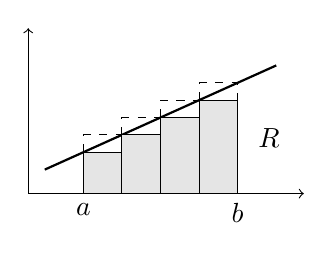
\begin{tikzpicture}[scale=.7]\draw[->](0,0)--(5,0);\draw[->](0,0)--(0,3);\draw[thick,domain=.3:4.5]plot(\x,{.3+.45*\x});\foreach \a/\b in {1/1.7,1.7/2.4,2.4/3.1,3.1/3.8}{\draw[fill=gray!20](\a,0)rectangle(\b,{.3+.45*\a});\draw[dashed](\a,{.3+.45*\a})rectangle(\b,{.3+.45*\b});}\node[below]at(1,0){$a$};\node[below]at(3.8,0){$b$};\node[right]at(4,1){$R$};\end{tikzpicture}\end{center}
% Pagina originale 80
\pagina{80}\tit{Osservazioni sugli infimi e supremi}
Se $A\subset B\subset\R$, $\inf B\le\inf A\le\sup A\le\sup B$.
Se $A\subset B\subset C\subset\R$, $f:C\to\R$ continua, allora
\[f(A)\subset f(B)\subset f(C)\subset\R,\qquad
\inf_{t\in A}f(t)=\inf f(A)\ge\inf f(B)=\inf_{t\in B}f(t).\]
\[M_i:=\sup_{t\in[t_{i-1},t_i]}f(t)\le\sup f\in\R\Longrightarrow M_i\in\R,\]
\[m_i:=\inf_{t\in[t_{i-1},t_i]}f(t)\ge\inf f\in\R\Longrightarrow m_i\in\R.\]
\tit{Relazioni tra somme inferiori e superiori}
\[A:=\{s(f,D):D\in\mathcal D([a,b])\}\subset\R,\quad
B:=\{S(f,D):D\in\mathcal D([a,b])\}\subset\R.\]
\textbf{1.} $A\ne\varnothing$, $B\ne\varnothing$.
\textit{Dimostrazione.} $\{a,b\}\in\mathcal D([a,b])$.
\textbf{2.} $A$ e $B$ sono separati: $\forall x\in A,\forall y\in B$, $x\le y$.
\textit{Dimostrazione.} Per una stessa suddivisione $\bar D$,
\[s(f,\bar D)\le S(f,\bar D),\qquad
\sum_{i=1}^n m_i(t_i-t_{i-1})\le\sum_{i=1}^n M_i(t_i-t_{i-1}),\]
poiché $m_i\le M_i$ per ogni $i$.
% Pagina originale 81
\pagina{81}
$D_1,D_2\in\mathcal D([a,b])$; consideriamo il caso particolare $D_2\subset D_1$ (nel manoscritto $|D_1|\ge|D_2|$ indica qui cardinalità).
\[s(f,D_2)\le s(f,D_1)\le S(f,D_1)\le S(f,D_2).\]
Sia $D_1=D_2\cup\{\bar t\}$, $\bar t\in(a,b)$ nuovo punto, posto fra $t_3$ e $t_n$ nel disegno.
\begin{center}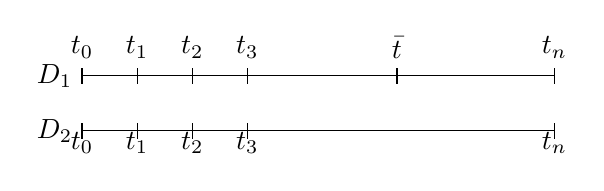
\begin{tikzpicture}\draw(0,0)--(6,0);\draw(0,-.7)--(6,-.7);\foreach \x/\lab in {0/t_0,.7/t_1,1.4/t_2,2.1/t_3,6/t_n}{\draw(\x,-.1)--(\x,.1)node[above]{$\lab$};\draw(\x,-.8)--(\x,-.6)node[below]{$\lab$};}\draw(4,-.1)--(4,.1)node[above]{$\bar t$};\node[left]at(0,0){$D_1$};\node[left]at(0,-.7){$D_2$};\end{tikzpicture}\end{center}
Gli addendi degli intervalli invariati si cancellano. Detto $\bar m=\inf_{[t_3,t_n]}f$, $\bar m_1=\inf_{[t_3,\bar t]}f$ e $m_n=\inf_{[\bar t,t_n]}f$, si deve verificare
\[\bar m_1(\bar t-t_3)+m_n(t_n-\bar t)\ge\bar m(t_n-t_3).\]
Nel caso illustrato $\bar m_1=\bar m$:
\begin{align*}
\bar m(\bar t-t_3)+(\bar m+(m_n-\bar m))(t_n-\bar t)
&=\bar m(\bar t-t_3)+\bar m(t_n-\bar t)+(m_n-\bar m)(t_n-\bar t)\\
&=\bar m(t_n-t_3)+(m_n-\bar m)(t_n-\bar t)\ge\bar m(t_n-t_3),
\end{align*}
perché $(m_n-\bar m)(t_n-\bar t)\ge0$.
Infatti $[\bar t,t_n]\subset[t_3,t_n]$, dunque
\[m_n=\inf_{[\bar t,t_n]}f\ge\inf_{[t_3,t_n]}f=\bar m.\]
\nota{Pagina 81: il disegno e il calcolo trattano l'aggiunta di un punto; nel caso generale si utilizza la suddivisione comune $D_1\cup D_2$.}
% Pagina originale 82
\pagina{82}\tit{Integrabilità secondo Riemann}
$A$ e $B$ contigui, cioè $\sup A=\inf B$, implica $f$ integrabile.
\[\int_a^b f(x)\,dx:=\sup A=\inf B.\]
\tit{Integrale di una funzione costante}
\[\int_a^b f(x)\,dx=c(b-a),\qquad f(x)=c\quad\forall x\in\operatorname{dom}f.\]
\tit{Continuità implica integrabilità}
\[f\in C^0([a,b])\Longrightarrow f\in\mathcal R([a,b]),\]
\[\mathcal R([a,b]):=\{f:[a,b]\to\R\mid f\text{ limitata e integrabile in }[a,b]\}.\]
\tit{Ampiezza di una suddivisione}
Per $D\in\mathcal D([a,b])$, $|D|$ è il massimo delle ampiezze:
\[|D|=\max_{i\in\{1,\ldots,n\}}(t_i-t_{i-1}).\]
\textit{Osservazione.} Per ogni $\varepsilon>0$ esiste $D$ con $|D|<\varepsilon$: si prende $n$ tale che $(b-a)/n<\varepsilon$, cioè $b-a<n\varepsilon$.
\begin{align*}
A,B\text{ contigui}&\iff\forall\varepsilon>0\ \exists x\in A,y\in B:\ y-x<\varepsilon\\
&\iff\forall\varepsilon>0\ \exists D_1,D_2:\ S(f,D_1)-s(f,D_2)<\varepsilon\\
&\iff\forall\varepsilon>0\ \exists D:\ S(f,D)-s(f,D)<\varepsilon.
\end{align*}
Quindi $f\in\mathcal R([a,b])$ se e solo se per ogni $\varepsilon>0$ esiste $D\in\mathcal D([a,b])$ con $S(f,D)-s(f,D)<\varepsilon$.
% Pagina originale 83
\pagina{83}\tit{Funzioni crescenti integrabili}
$f$ crescente implica $f$ integrabile.
Per $\varepsilon>0$, consideriamo $\varepsilon/(f(b)-f(a))$; prendiamo $D$ con $|D|<\varepsilon/(f(b)-f(a))$.
\begin{align*}
s(f,D)&=\sum_{i=1}^n m_i(t_i-t_{i-1})=\sum_{i=1}^n f(t_{i-1})(t_i-t_{i-1}),\\
S(f,D)&=\sum_{i=1}^n M_i(t_i-t_{i-1})=\sum_{i=1}^n f(t_i)(t_i-t_{i-1}),\\
S(f,D)-s(f,D)&=\sum_{i=1}^n(f(t_i)-f(t_{i-1}))(t_i-t_{i-1})\\
&<\frac\varepsilon{f(b)-f(a)}\sum_{i=1}^n(f(t_i)-f(t_{i-1}))\\
&=\frac\varepsilon{f(b)-f(a)}[f(t_1)-f(a)+f(t_2)-f(t_1)+\cdots+f(b)-f(t_{n-1})]\\
&=\frac\varepsilon{f(b)-f(a)}(f(b)-f(a))=\varepsilon.
\end{align*}
Quindi $S(f,D)-s(f,D)<\varepsilon$.
\nota{Pagina 83: se $f(b)=f(a)$, la funzione crescente è costante e il risultato segue dal caso già trattato.}
\tit{Proprietà}
\begin{enumerate}\item Additività: $\displaystyle\int_a^b f(x)\,dx=\int_a^c f(x)\,dx+\int_c^b f(x)\,dx$.
\item Linearità: per $\alpha,\beta\in\R$, $\displaystyle\int_a^b(\alpha f(x)+\beta g(x))\,dx=\alpha\int_a^b f(x)\,dx+\beta\int_a^b g(x)\,dx$.
\item $f\le g$ in $[a,b]$ implica $\displaystyle\int_a^b f(x)\,dx\le\int_a^b g(x)\,dx$.\end{enumerate}
\nota{Pagina 83: il manoscritto indica un'equivalenza nell'ultima proprietà; il confronto degli integrali non implica in generale il confronto puntuale delle funzioni.}
% Pagina originale 84
\pagina{84}
\textbf{4.} $f\ge0\Longrightarrow\int_a^b f(x)\,dx\ge0$.
\textbf{5.} $\displaystyle m(b-a)\le\int_a^b f(x)\,dx\le M(b-a)$.
\tit{Media integrale}
\[m(b-a)\le\int_a^b f(x)\,dx\le M(b-a),\qquad
m\le\frac1{b-a}\int_a^b f(x)\,dx\le M.\]
Se $f\in C^0([a,b])$, esiste $c\in[a,b]$ tale che
\[f(c)=\frac{\int_a^b f(x)\,dx}{b-a},\]
grazie al teorema dei valori intermedi e al teorema di Weierstrass.
\tit{Teorema fondamentale del calcolo integrale}
\textit{Ipotesi.} $f\in C^0([a,b])\subset\mathcal R([a,b])$, $x_0\in[a,b]$.
\[F_{x_0}(x):=\int_{x_0}^x f(u)\,du,\qquad F_{x_0}:[a,b]\to\R.\]
La funzione integrale è nulla in $x_0$.
\textit{Tesi.} $F$ derivabile e $F'(x)=f(x)$.
\textit{Dimostrazione.} Per $h\to0^+$,
\begin{align*}
\frac{F(x+h)-F(x)}h&=\frac{\int_{x_0}^{x+h}f(u)\,du-\int_{x_0}^xf(u)\,du}{h}\\
&=\frac{\int_{x_0}^xf(u)\,du+\int_x^{x+h}f(u)\,du-\int_{x_0}^xf(u)\,du}{h}
=\frac{\int_x^{x+h}f(u)\,du}{h}.
\end{align*}
Esiste $c\in(x,x+h)$ tale che $\displaystyle f(c)=\frac{\int_x^{x+h}f(u)\,du}{h}$.
% Pagina originale 85
\pagina{85}
$c\in(x,x+h)$ implica $c\to x$ quando $h\to0^+$. Quindi $f(c)\to f(x)$ e
\[F'(x)=\lim_{h\to0^+}\frac{\int_x^{x+h}f(u)\,du}{h}=f(x).\]
\tit{Corollario}
\textit{Ipotesi.} $f\in C^0([a,b])$, $G:[a,b]\to\R$ primitiva di $f$.
\textit{Tesi.}
\[\int_a^bf(u)\,du=G(b)-G(a)=\left.G(x)\right|_a^b.\]
\textit{Dimostrazione.} $F_a(x)=\int_a^x f(u)\,du$. Le primitive differiscono per una costante $c$:
\[G(b)=\int_a^bf(u)\,du+c,\qquad G(a)=0+c,\qquad
G(b)=\int_a^bf(u)\,du+G(a).\]
\tit{Integrazione per parti}
\[\int_a^b f(u)g'(u)\,du=\left.f(u)g(u)\right|_a^b-\int_a^bf'(u)g(u)\,du.\]
\tit{Integrazione per sostituzione}
\[\int_a^bf(x)\,dx=\int_{g(a)}^{g(b)}f(g(t))g'(t)\,dt.\]
\nota{Pagina 85: gli estremi sono riportati come nel manoscritto. La formula usuale è $\int_{g(a)}^{g(b)}f(x)\,dx=\int_a^bf(g(t))g'(t)\,dt$.}
\tit{Osservazioni sulla simmetria}
\[\int_{-a}^a f(u)\,du=2\int_0^af(u)\,du\quad\text{se }f(-x)=f(x)\quad(\text{pari}),\]
\[\int_{-a}^a f(u)\,du=0\quad\text{se }f(-x)=-f(x)\quad(\text{dispari}).\]
% Pagina originale 86
\pagina{86}
\textit{Dimostrazione, caso pari.}
\begin{align*}
\int_{-a}^af(u)\,du&=\int_{-a}^0f(u)\,du+\int_0^af(u)\,du\\
&=\int_a^0-f(-u)\,du+\int_0^af(u)\,du\\
&=-\int_a^0f(u)\,du+\int_0^af(u)\,du=2\int_0^af(u)\,du.
\end{align*}
\textit{Caso dispari.}
\begin{align*}
\int_{-a}^af(u)\,du&=\int_a^0-f(-u)\,du+\int_0^af(u)\,du\\
&=\int_a^0f(u)\,du+\int_0^af(u)\,du
=\left(\int_0^af(u)\,du\right)(1-1)=0.
\end{align*}
\tit{Continuità della funzione integrale}
\textit{Tesi.} $F_{x_0}:[a,b]\to\R$ appartiene a $C^0([a,b])$.
\textit{Dimostrazione.} Sia $\bar x\in[a,b]$; vogliamo $\lim_{x\to\bar x}(F_{x_0}(x)-F_{x_0}(\bar x))=0$.
\[\lim_{x\to\bar x}\left[\int_{x_0}^xf(u)\,du-\int_{x_0}^{\bar x}f(u)\,du\right]
=\lim_{x\to\bar x}\int_{\bar x}^xf(u)\,du=0.\]
\nota{Pagina 86: nell'ultima riga del manoscritto l'integrale compare anche con estremi $x,\bar x$; il limite è comunque zero.}
